Ahora que tenemos planificadas la gran mayoría de tareas principales y a más alto nivel, vamos a empezar con el desarrollo como tal de la aplicación. En esta sección presentaremos el logo de la app junto con el nombre y los diseños de las principales interfaces. 

\subsubsection{Logo de la aplicación y nombre}

Una de las primeras cosas en las que pensamos cuando escuchamos aplicación móvil es en el nombre y el logo de las grandes aplicaciones. En la época actual los logos tienen a ser minimalistas, simples y con colores pastel y suaves. Así mismo los nombres de las aplicaciones tienden a ser cortos, ya que los dispositivos móviles suelen tener un tamaño reducido y no se pueden meter frases largas. 

\subsubsection*{Logo}

Los dos diseños iniciales para el logo de la aplicación fueron los siguientes: 

\begin{multicols}{2}
    \begin{figure}[H]
        \centering
        
\includegraphics[scale=0.8]{imagenes/diseno/logo1.png}
        \caption{Diseño 1 del logo de la aplicación}
        \label{fig:logo1}
    \end{figure}
    
    \begin{figure}[H]
        \centering
        
\includegraphics[scale=0.8]{imagenes/diseno/logo2.png}
        \caption{Diseño 1 del logo de la aplicación}
        \label{fig:logo2}
    \end{figure}
\end{multicols}

Pero después de una reunión con el cliente final, se llego a la conclusión de que el logo debería de ir mas por el estilo de la paleta:

\begin{figure}[H]
    \centering
    
\includegraphics[scale=0.3]{imagenes/diseno/logo3.png}
    \caption{Diseño final del logo de la aplicación}
    \label{fig:logo3}
\end{figure}

\subsubsection*{Nombre}

En la sección anterior ya hemos dejado ver cual iba a ser el nombre de la aplicación. Una de las ideas iniciales era:
\begin{itemize}
    \item \textbf{PigemtsDB}: pero ni al cliente ni al tutor del TFG les convencía esta opción, ya que al contener la acortación DB, procedente de Data Base incluía unas connotaciones un poco más técnicas.
\end{itemize}

Al final se ha dejado como \textbf{Pigment Studio} ya que tiene un significado ligeramente más general y no restringe a ningún tipo de colectivos. 

Es un nombre corto y que haces una buena referencia a lo que el usuario se va a encontrar cuando abra la aplicaicón, que no es más que un estudio bastante avanzado y claro de los diferentes pigmentos que tenemos en el mundo. 

\subsubsection{Diseño de las primeras interfaces}

Una de las partes más críticas cuando estamos desarrollando aplicaciones que va a utilizar el usuario final es la interfaz que van a tener que usar. Va a ser una pantalla contra la que el usuario va a interactuar bastante a menudo, por lo tanto tiene que ser cómoda, clara y sencilla. Algunas de las normas que tienen que tener el diseño de interfaces para que el usuario tenga una buena experiencia (UX) las podemos encontrar en la siguiente lista \textcolor{red}{buscar en la bibliografía de IPC algo sobre el diseño de interfaces de usuario y citar un par de libros}: 
\begin{itemize}
   \item 
\end{itemize}

Las principales interfaces que vamos a encontrar en nuestro sistema son las siguientes, junto con una descripción de lo que harán. 

\subsubsection*{Menú Principal}

En el menú principal de la aplicación podremos encontrar las diferentes opciones que nos presenta para explotar la base de datos de la manera más adecuada. Entre ellos los botones que nos podemos encontrar (recordar que solo son bocetos):
\begin{itemize}
    \item \textbf{Pigmentos}: en esta sección encontraremos una lista con todos los pigmentos que tenemos en la base de datos con algunas características en miniatura.
    \item \textbf{Consulta Simple}: nos permitirá realizar las principales consultas, que son por color y por el elemento químico principal del pigmento en cuestión. 
    \item \textbf{Consulta Avanzada}: nos permitirá realizar búsquedas más avanzadas, como por las coordenadas tricrómicas de un pigmento o por determinadas características de las gráficas de los mismos.
    \item \textbf{Gráficas}: mostrará al usuario una lista de las diferentes gráficas que se disponen de cada pigmento.
    \item \textbf{Añadir Pigmento}: el usuario podrá añadir un nuevo pigmento a la base de datos, en el caso de que se disponga de los datos suficientes para hacerlo. 
\end{itemize}

Podemos ver la vista del menú principal en la \textbf{Figura \ref{fig:menuPrincipal}}

\newpage
\begin{multicols}{2}
    \begin{figure}[H]
    \centering
    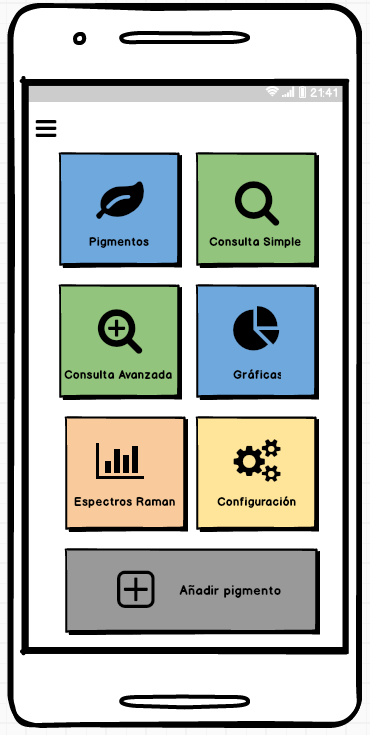
\includegraphics[scale=0.6]{imagenes/diseno/main.png}
    \caption{Menú principal de la aplicación}
    \label{fig:menuPrincipal}
    \end{figure}
    
    \begin{figure}[H]
    \centering
    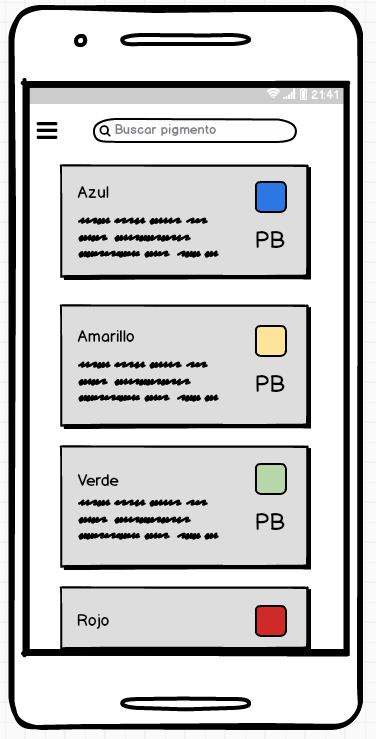
\includegraphics[scale=0.6]{imagenes/diseno/lista.png}
    \caption{Lista principal con todos los pigmentos del sistema}
    \label{fig:listaPigmentos}
    \end{figure}
\end{multicols}

\subsubsection*{Vista rápida de pigmentos}

Si el usuario pulsa sobre el botón de pigmentos, entonces lo que se va a encontrar es una sencilla lista con todos los pigmentos que se encuentran disponibles en el sistema. La entrada de cada pigmento constará del nombre del mismo, un color aproximado, para que se le haga mas visual al usuario, junto con una breve descripción y en miniatura el elemento químico principal que compone dicho pigmento. Podemos observar dicho menú en la \textbf{Figura \ref{fig:listaPigmentos}}. En esta vista el usuario puede buscar por nombre un determinado pigmento, puede conseguir esto introduciendo el nombre del mismo en la barra superior que tenemos en el menú.

\subsubsection*{Información de los pigmentos}

Una vez que en la pantalla que hemos presentado anteriormente, el usuario pulsa sobre uno de los pigmentos, el sistema muestra toda la información detalla del mismo según la \textbf{Figura \ref{fig:infoPigmentos}}

\newpage
\begin{multicols}{2}
    \begin{figure}[H]
    \centering
    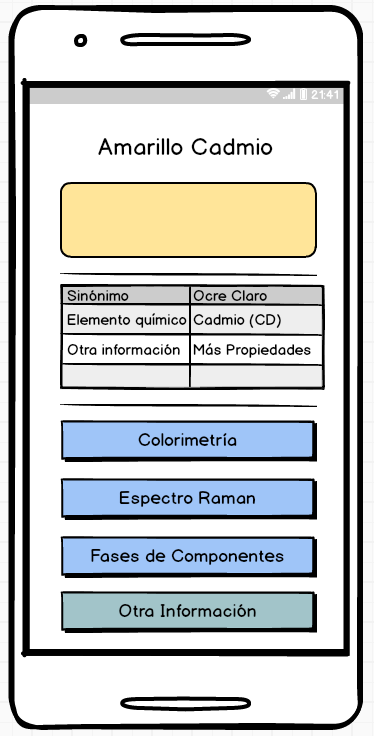
\includegraphics[scale=0.6]{imagenes/diseno/inforPigmento.png}
    \caption{Información de los pigmentos}
    \label{fig:infoPigmentos}
    \end{figure}
    
    \begin{figure}[H]
    \centering
    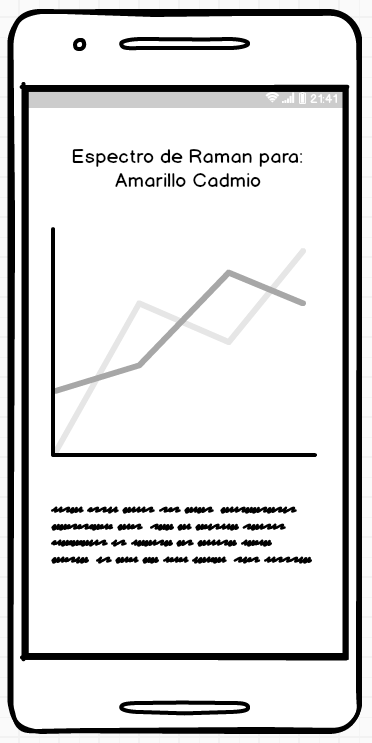
\includegraphics[scale=0.6]{imagenes/diseno/infoGraficas.png}
    \caption{Información gráficas de pigmentos}
    \label{fig:infoGraficas}
    \end{figure}
\end{multicols}

\subsubsection*{Consulta Simple - Opción 1}

Volviendo al menú principal, si el usuario pulsa sobre el botón de consulta simple entonces se le muestran las diferentes opciones, que en este caso solo son 3, una es la búsqueda por color, otra la búsqueda por un elemento químico y la tercera es la opción que tendríamos en el menú principal de verlos todos. Además una vez que el usuario pulsa sobre una de las dos opciones, el sistema le muestra los diferentes formularios para ejecutar la búsqueda. 

En esta sección tenemos que presentar dos bocetos diferentes, que son los que se habían pensado en el principio, y luego se darán más detalles para decir con cual nos hemos decantado. 

Podemos ver los primeros bocetos en las Figuras siguientes:

\newpage
\begin{multicols}{3}
    \begin{figure}[H]
    \centering
    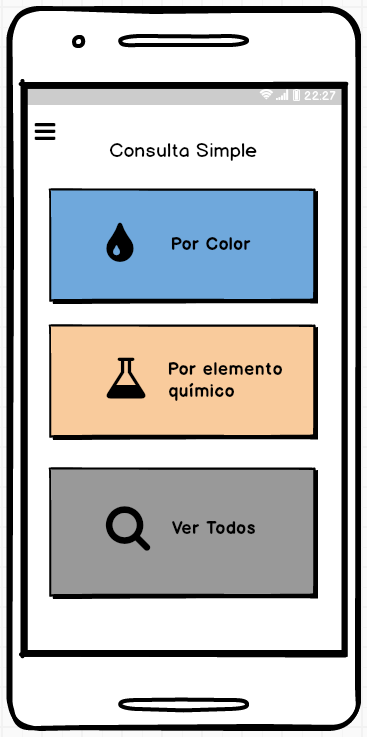
\includegraphics[scale=0.5]{imagenes/diseno/simpleQuery.png}
    \caption{Menú para hacer una consulta simple}
    \label{fig:consultaSimple}
    \end{figure}
    
    \begin{figure}[H]
    \centering
    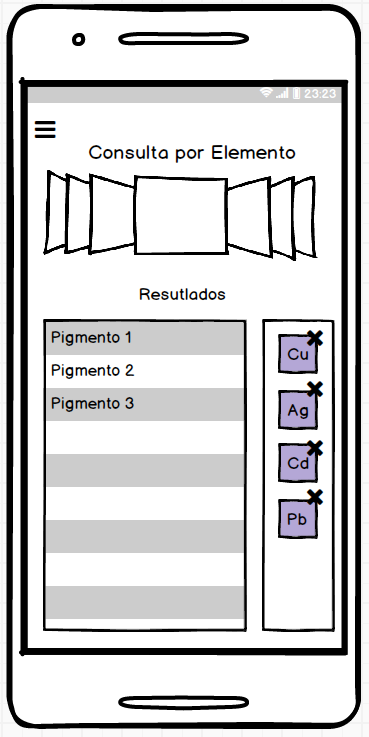
\includegraphics[scale=0.5]{imagenes/diseno/elementos1.png}
    \caption{Menú de selección de colores}
    \label{fig:consultaColores}
    \end{figure}
    
    \begin{figure}[H]
    \centering
    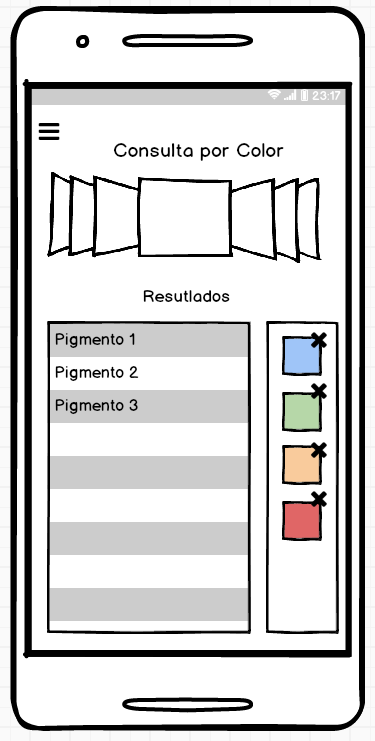
\includegraphics[scale=0.5]{imagenes/diseno/color1.png}
    \caption{Menú de selección de elementos}
    \label{fig:consultaElementos}
    \end{figure}
\end{multicols}

En la \textbf{Figura \ref{fig:consultaSimple}} podemos ver el menú principal que hemos descrito anteriormente, donde el usuario elije el tipo de búsqueda que quiere realizar. Mientras que en la \textbf{Figura \ref{fig:consultaColores}} podemos ver la selección de colores y en la \textbf{Figura \ref{fig:consultaElementos}} podemos ver como sería la pantalla de selección de elementos. 

La ventaja que tienen estas interfaces es que puedes un solo diseño de la vista de la aplicación para dos funcionalidades diferentes. Además es más dinámica ya que evita tener que pulsar tantos botones como las opciones que mostraremos a continuación. El usuario simplemente desliza en busca de los colores o elementos que quiere, va pulsando sobre ellos, dichos elementos se van añadiendo a la lista vertical de la derecha, y la lista de resultados se va actualizando automáticamente en función de los filtros introducidos. 

\subsubsection*{Consulta Simple - Opción 2}

Sin embargo en las \textbf{Figuras \ref{fig:consultaColores1}} y \textbf{Figuras \ref{fig:consultaElementos1}} podemos ver como era otra de las ideas iniciales para estas consultas.

\newpage
\begin{multicols}{2}
    \begin{figure}[H]
    \centering
    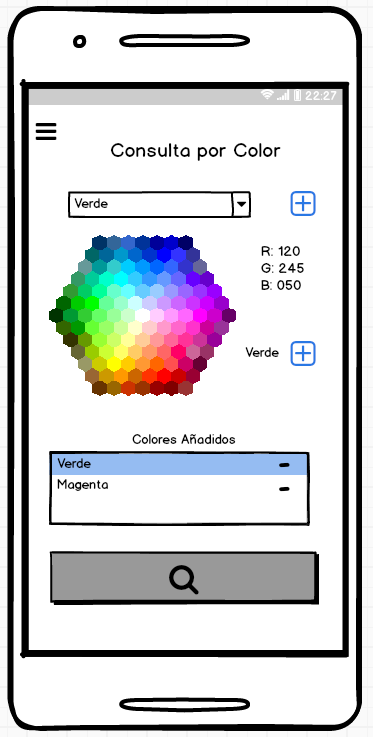
\includegraphics[scale=0.6]{imagenes/diseno/porColor.png}
    \caption{Menú de selección de colores}
    \label{fig:consultaColores1}
    \end{figure}
    
    \begin{figure}[H]
    \centering
    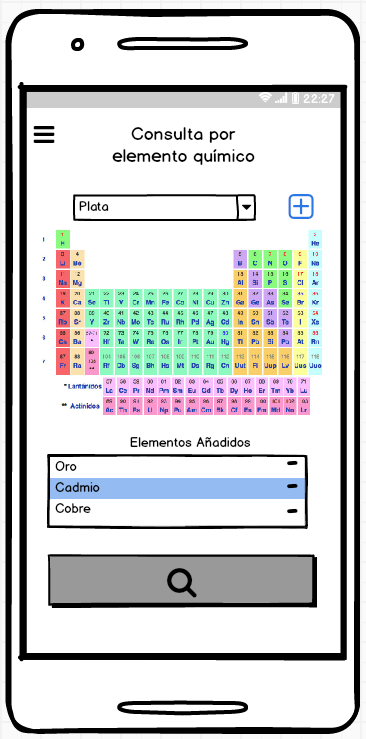
\includegraphics[scale=0.6]{imagenes/diseno/porElemento.png}
    \caption{Menú de selección de elementos}
    \label{fig:consultaElementos1}
    \end{figure}
\end{multicols}

Las desventajas que podemos encontrar al diseñar esta interfaz son varias. Primero es menos dinámica que la opción anterior ya que el usuario tiene que hacer más pulsaciones en la pantalla para obtener el mismo resultado, además de que tiene más pantallas intermedias, ya que se tienen que mostrar los resultados en una vista diferente. Otra de las desventajas desde el punto de vista de desarrollo es que requieren funcionalidades diferentes, en una tendríamos que añadir un selector de color e introducir cosas más específicas de este elemento mientras que la otra opción tendríamos que ingeniarnos un selector de elementos químicos, lo cual puede ser complicado. La opción anterior unifica estas opciones, ya que saca los colores y los elementos de una base de datos y solo tiene que cargar la información para que el usuario la elija como filtro de la búsqueda. 

Recordamos que las figuras anteriormente presentadas son solo bocetos de la aplicación. La idea es que la aplicación final quede de manera aproximada a como se ha mostrado, pero por problemas de desarrollo, tiempo u otras causas es posible que los resultados finales se vean afectados o no sean completamente fieles a los presentados en las figuras anteriores. 

\subsubsection*{Reportar Bug}

Esta pantalla no tiene mucha importancia a nivel de funcionalidad, pero si que la considero bastante importante a nivel de peticiones de cambio futuras y cuyo objetivo es mejorar la aplicación el tiempo. 

Los reportes de fallos o bugs de la aplicación, que sea reportados por los usuarios serán almacenados en un servidor central que gestionará una base de datos de fallos y bugs. Esta información se mandará de manera completamente anónima por la red, y no se almacenará ningún posible dato del usuario. 

La pantalla que tengo pensada para implementar esta funcionalidad la podemos observar en la \textbf{Figura \ref{fig:bugreport}}

\begin{figure}[H]
\centering
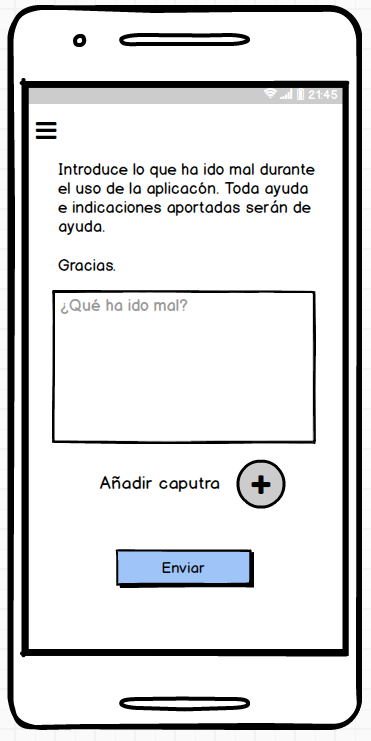
\includegraphics[scale=0.6]{imagenes/diseno/bugreport.png}
\caption{Menú de reporte de fallos}
\label{fig:bugreport}
\end{figure}
